\subsection{Context Clue Extraction Services}
%Bigrams 
During the background chapter we emphasized the importance of context and how much it can affect the disambiguation accuracy for both, automatic and manual annotation systems. Referring back to the work-flow presented in the diagram in Figure \ref{fig:workflow}, contextual clues are extracted by following a three step process.

The process starts by removing all stop words in the sentences where the entity mentions are part of. After the stop words have been removed from the sentences, the \textit{collocation generation algorithm} is performed on those sentences. Collocations, according to Colson et al. \cite{52} represent the occurrence of two or more words within a short proximity between each other in text. They also argues that collocations are more likely to occur as fixed expressions such as compound nouns, proper nouns, idioms, noun-adjective combination, adjective-noun combination, verb-noun, well known song or film titles. The collocation generation algorithm follows these principles when deciding to keep a collocation from the sentence or not. Since we are dealing with analysis of grammatical structures in the sentence, part-of-speech tagging is a crucial step to be performed at this stage. 

After having extracted all potential collocations from the sentence provided as input data to the service, the next step is to associate these collocations as contextual clues to each and every entity. However, not every identified collocation within the sentence can be a useful context clue for the entity that is also part of that sentence. Previous studies have used a context window size of 4, which means that they take four preceding and four subsequent words from the sentence where the target entity occurs \cite{35}. The number 4 has been chosen because the accuracy of sense resolution does not improve when more than 4 words around the target word are considered. However, recent studies argue that the context windows size around the ambiguous target entity is dependent on the nature of the word itself \cite{35}. Our solution to this problem is increasing the context window size depending on how ambiguous the target word is. The ambiguity of a target entity is defined by the number of potential candidates extracted from the \ac{kb}. The more candidates are generated for the target entity, the higher the level of ambiguity. We believe that this represents an accurate metric on deciding the context size of the target entity. 

Since collocations can be a combination of more than two words, we have decided to keep only collocations that are composed of two words (i.e. bigrams). This decision is influenced on the findings acquired by Mihalcea and Rada \cite{36}. They observed that in terms of words in context, bigrams seem to be more effective than simple keywords and other combinations larger than two.In addition to the collocations which are considered as clues to help summarize the context in which the target word occurs, neighbour entities also also fall into this category. Since the algorithm has information on the exact position of each entity in the sentence (by maintaining a starting and ending index), we are able to decide which (other) entities are in close proximity to the target entity. Usually all identified entities that are part of the same sentence as the target entity are considered as neighbor entities. In some cases, when the sentence is short, the algorithm looks for neighbor entities in the preceding and subsequent sentences. The algorithm maintains a constraint on which it bases its logic whether to consider keeping or discarding a neighbor entity for the target entity. The constraint is basically a calculated word distance between the target entity and all other potential neighbor entities. 

After the local contextual clues have been extracted by our internal microservice, the last step is the extraction of document keywords. Document keywords are used to represent the theme or topic of the document, and might help in the disambiguation process in addition to local contextual clues. In this stage, Alchemy API is queried which extracts the most important keywords from a document. These keywords are associated as context clues to all identified entities in the same document whereas local context clues are distinct from one entity to another. Figure \ref{fig:context-clue} illustrates an example of a paragraph and the corresponding results after running the context clue extraction service. In this example, the target entity for which the context clues are to be associated is highlighted in red. The legend illustrated as a table in the example figure explains the meaning of the different colors. In cases where the words are underlined and highlighted with different colors, it means that the word combination has multiple purposes. For example "New York" from the illustrative paragraph in Figure \ref{fig:context-clue} is considered a neighbor entity to G1 (the target entity) in addition to being a keyword that contributes to understanding the meaning of the complete paragraph.


\begin{figure}[]
  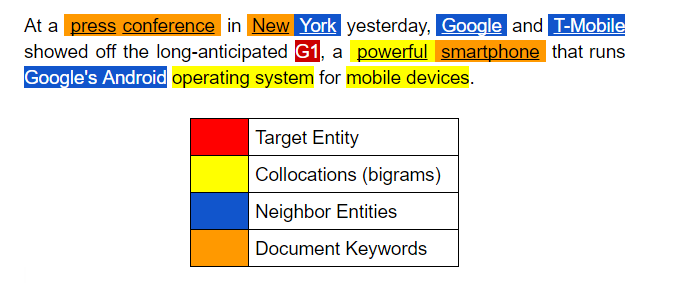
\includegraphics[width=\linewidth]{figures/context-clues.png}
  \caption{An example of a paragraph and the different contextual clues extracted from the service}
  \label{fig:context-clue}
\end{figure}